\def\year{2015}
\documentclass[letterpaper]{article}
\usepackage{aaai}
\usepackage{times}
\usepackage{helvet}
\usepackage{courier}
\usepackage{graphicx}
\usepackage{url}
\setlength\titlebox{3in}
\frenchspacing
\copyrighttext{Copyright 2015, California Institute of Technology.
All rights reserved.}
\setlength{\pdfpagewidth}{8.5in}
\setlength{\pdfpageheight}{11in}
\pdfinfo{
%/Title (Towards Automatic Generation of a Mars Target Encyclopedia)
/Title (Creating a Mars Target Encyclopedia by Extracting Information from
the Planetary Science Literature)
/Author (Kiri L. Wagstaff, Nina Lanza, Ellen Riloff, Chris Mattmann, Paul Ramirez)}
\setcounter{secnumdepth}{2}  
 \begin{document}
% The file aaai.sty is the style file for AAAI Press 
% proceedings, working notes, and technical reports.
%
%\title{Towards Automatic Generation of a Mars Target Encyclopedia}
\title{Creating a Mars Target Encyclopedia by Extracting Information from
the Planetary Science Literature}
\author{Kiri L. Wagstaff \\
Jet Propulsion Laboratory\\
California Institute of Technology\\
4800 Oak Grove Drive, Pasadena, CA 91109\\
{\tt kiri.l.wagstaff@jpl.nasa.gov}
\And
Ellen Riloff\\
School of Computing\\
University of Utah\\
Salt Lake City, UT 84112\\
{\tt riloff@cs.utah.edu}
\And
Nina L. Lanza\\
Los Alamos National Laboratory \\
Los Alamos, NM  87545\\
{\tt nlanza@lanl.gov}
\AND
Chris A. Mattmann\\ 
\normalsize Jet Propulsion Laboratory\\
\normalsize California Institute of Technology\\
\normalsize 4800 Oak Grove Drive, Pasadena, CA 91109\\
\normalsize {\tt chris.a.mattmann@jpl.nasa.gov}
\And
Paul M. Ramirez\\
\normalsize Jet Propulsion Laboratory\\
\normalsize California Institute of Technology\\
\normalsize 4800 Oak Grove Drive, Pasadena, CA 91109\\
\normalsize {\tt paul.m.ramirez@jpl.nasa.gov}
}
\maketitle
\begin{abstract}
\begin{quote}
Staying up to date with the latest discoveries is a challenge in any
scientific field.  In planetary science, new observation targets on
the surface of Mars are identified and named every day, and new
publications announcing new discoveries and conclusions provide
frequent updates about these targets.
%
We are constructing a system that uses information extraction and
retrieval methods to mine the steadily growing body of planetary
science publications about Mars surface targets and automatically
construct a concise summary of what is known about each target.  The
Mars Target Encyclopedia will provide a central, continually updated
resource for use by planetary scientists and the interested public.
We describe our use of Tika, Sundance, and AutoSlog to extract and
summarize information, some of the challenges associated with this
domain, and our plans for maturing the system.
\end{quote}
\end{abstract}

\section{Introduction and Motivation}

The rovers that have been sent to Mars have been extraordinarily
active and productive.  The Mars Science Laboratory rover has
generated $>3500$ observation targets in three years, and the Mars
Exploration Rover Opportunity has generated even more over its
11+-year mission.  There are hundreds of associated scientific
publications reporting new discoveries.  The downside of this
productivity is that as the number of data and publications grow, it
becomes
% progressively more difficult 
% EMR: changed to be stronger. Change back if too strong!
nearly impossible
for any single person to read, understand, organize, and recollect the
amount of information available.  
% EMR: I commented out the sentences below because I'm not sure
% that the situation is so different from other scientific fields. New
% medical studies  and genomic research papers appear daily too. I've
% seen staggering statistics  on how rapidly the literature is
% growing, though I don't remember them offhand. :)
%% All researchers face the challenge
%% of staying up to date on new methods and advances in their field, but
%% Mars surface studies are particularly challenging because rather than
%% learning about a handful of new methods every few months or so
%% (through a new journal issue or a conference proceedings), the list of
%% newly identified targets and discoveries grows daily.

We focus on a specific challenge, which is that of staying up-to-date
with everything known (published) about identified surface targets on
Mars.  Each time an instrument (camera, spectrometer, laser, etc.) is
aimed at a target (soil, rock, formation, etc.), that target is given
a unique name.
%
Mission planners and planetary science researchers must be aware of an
increasing number of names, locations, and facts so that new
observations can be appropriately interpreted in the context of what
is already known.  For example, one might ask: Does the observation of
high manganese content at a particular location represent a
confirmation of an existing trend or an anomalous new discovery?

\begin{figure}
\centerline{\fbox{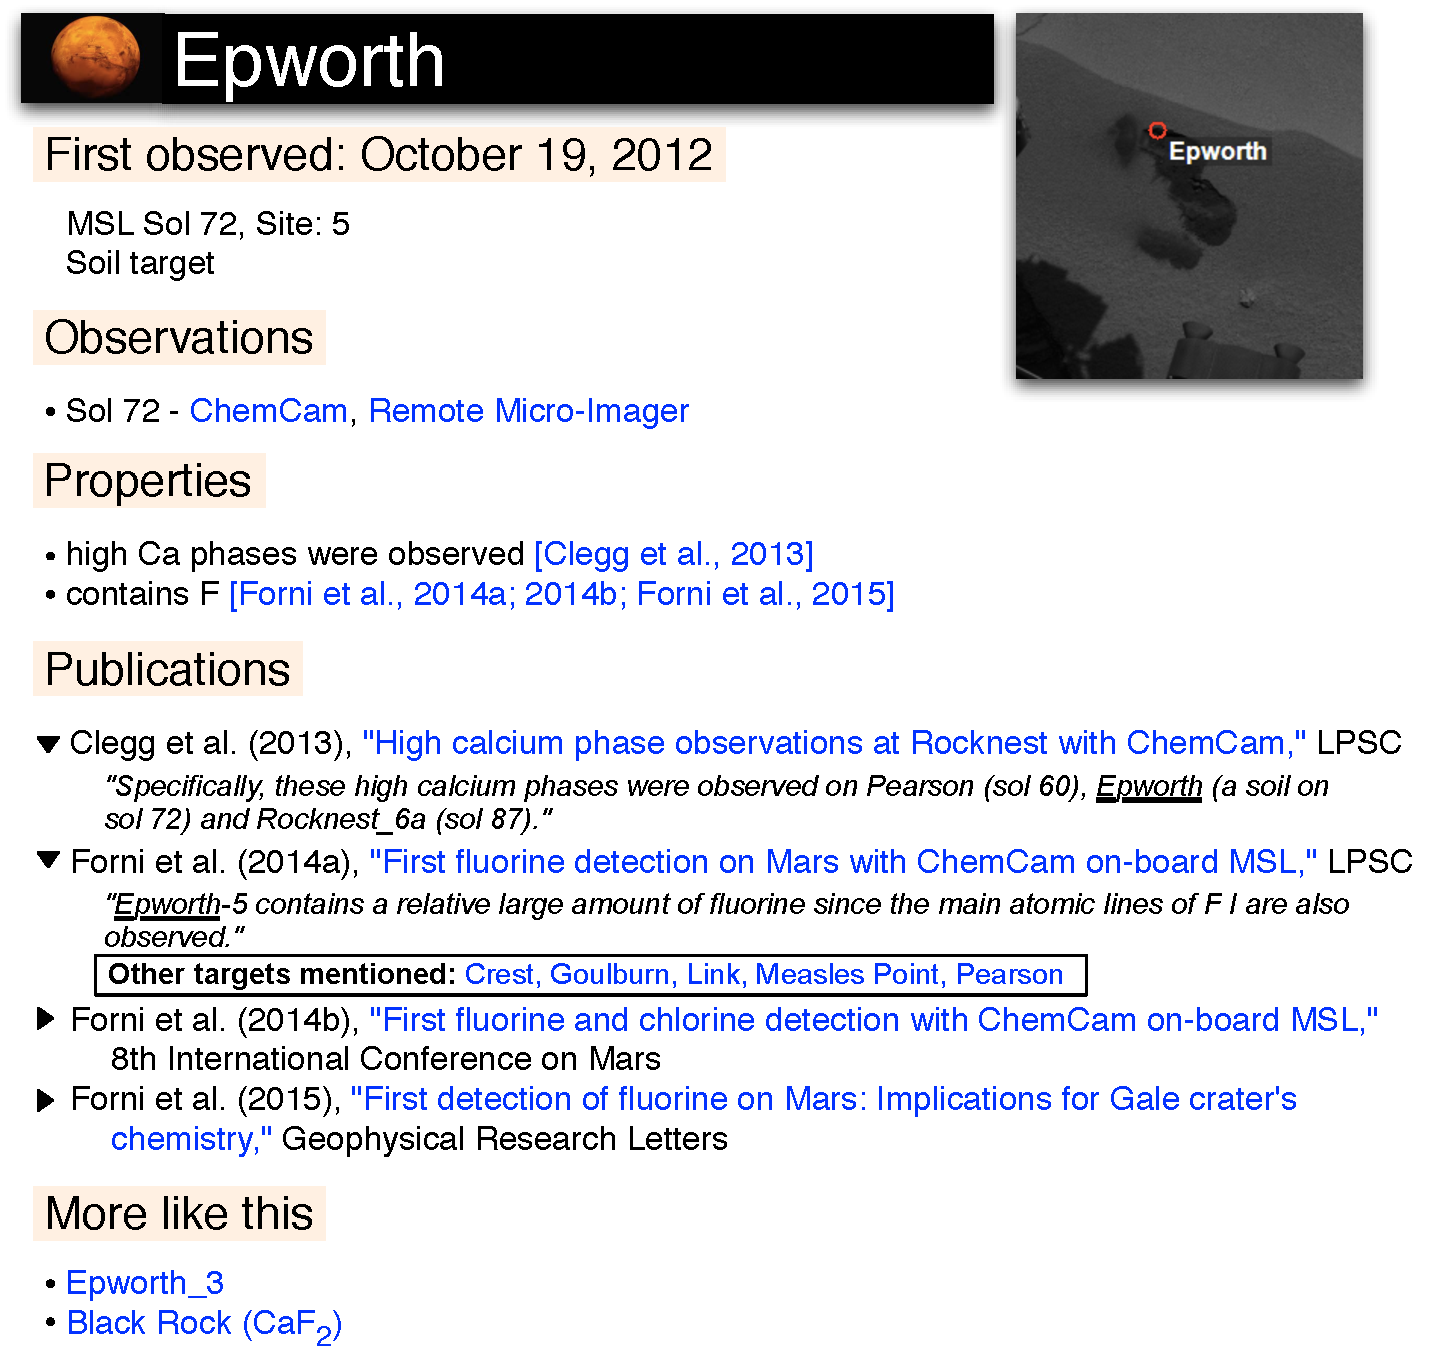
\includegraphics[width=3.25in]{fig/mte-epworth}}}
\caption{Example hand-constructed MTE entry for target
Epworth. Users can connect to the original observations, properties
that were extracted from scientific publications, and the publications
themselves.  Each publication provides excerpts with relevant context
and a list of other targets mentioned.}
\label{fig:epworth}
\end{figure}

Current text search tools cannot meet the knowledge needs of planetary
scientists and mission planners.  Mars surface target names have no
naming convention, and names are often borrowed from Earth locations
(e.g.,~``Cumberland,'' ``Ithaca''), people (e.g., ``Jake'',
``Darwin''), or apparent whimsy (``Frood,'' ``Worldbeater'').  Using
Google or journal text search interfaces with these names yields many
irrelevant results.
%Volume of data: MSL - XXXX papers published in 3 years; YYYY targets
%observed by ChemCam
This situation presents an opportunity for NLP and information
extraction (IE) and retrieval (IR) methods to make a major
contribution that can help advance the field of planetary science.
The number of targets, amount of data, and number of associated
publications are too large for a manual solution to be feasible. This
task also presents important challenges that can motivate advances in
IE that can benefit other domains.

We are working to construct a Mars Target Encyclopedia (MTE) that will
contain knowledge about Mars surface targets.  The MTE will provide
access to the data and publications associated with each target (see
Figure~\ref{fig:epworth} for a hand-constructed example).  Each entry
will also include a list of properties that were automatically
extracted from the publications, providing a high-level summary of
relevant knowledge.  The associated excerpts will be highlighted for
each publication, serving to (1) provide support for each of the
extracted properties and (2) enable users to quickly determine which
papers are of the most interest.  

The MTE project is in an early stage.  In this paper, we report on the
motivation, concept, approach, and early results that we have
obtained.  We also discuss the associated challenges that are of
interest to the NLP and IR communities, and we describe the next steps
that we will pursue.  

\section{Constructing a Mars Target Encyclopedia}

\subsection{Data Set Description}

For our initial study, we constructed a corpus that consists of all
papers presented at the 2015 Lunar and Planetary Science
Conference (LPSC)\footnote{Downloaded
from \url{http://www.hou.usra.edu/meetings/lpsc2015/}}. 
Each of the 1,991 papers is a maximum two-page extended abstract with a
common structure: title, authors with affiliations, a two-column main
body that may contain figures and/or tables, and references.  The
language is academic and makes heavy use of complex noun phrases and
parenthetical expressions.  The passive voice is often used.
% Todo: include examples

%The LPSC papers are provided in PDF format.  
We used the Apache Tika parser~\cite{mattmann:tika11} to read the PDF
files and convert them to plain text.  Four documents could not be
parsed by Tika, yielding 1,987 documents.  The number of extracted
words per document ranged from 142 to 2433.

% target list
We also obtained a seed list of Mars surface target names identified by
the ChemCam science team.  ChemCam is an instrument on the Mars
Science Laboratory (MSL) rover.  It fires a laser at rock or soil targets
and then uses a spectrometer to record the emitted energy at 6,144
wavelengths~\cite{maurice:chemcam12}.  The current list of all ChemCam
observations can be obtained
online\footnote{\url{http://pds-geosciences.wustl.edu/msl/msl-m-chemcam-libs-4_5-rdr-v1/mslccm_1xxx/document/msl_ccam_obs.csv}}.
The version we used contained 16,267 observations that spanned 656
distinct targets.

\subsection{Information Extraction Approach}

\begin{figure}
%\centerline{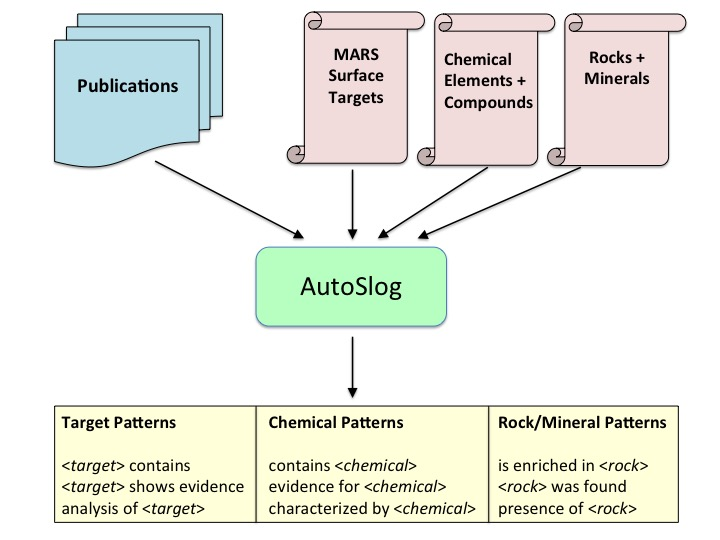
\includegraphics[width=3.5in]{fig/autoslog-process.jpg}}
\centerline{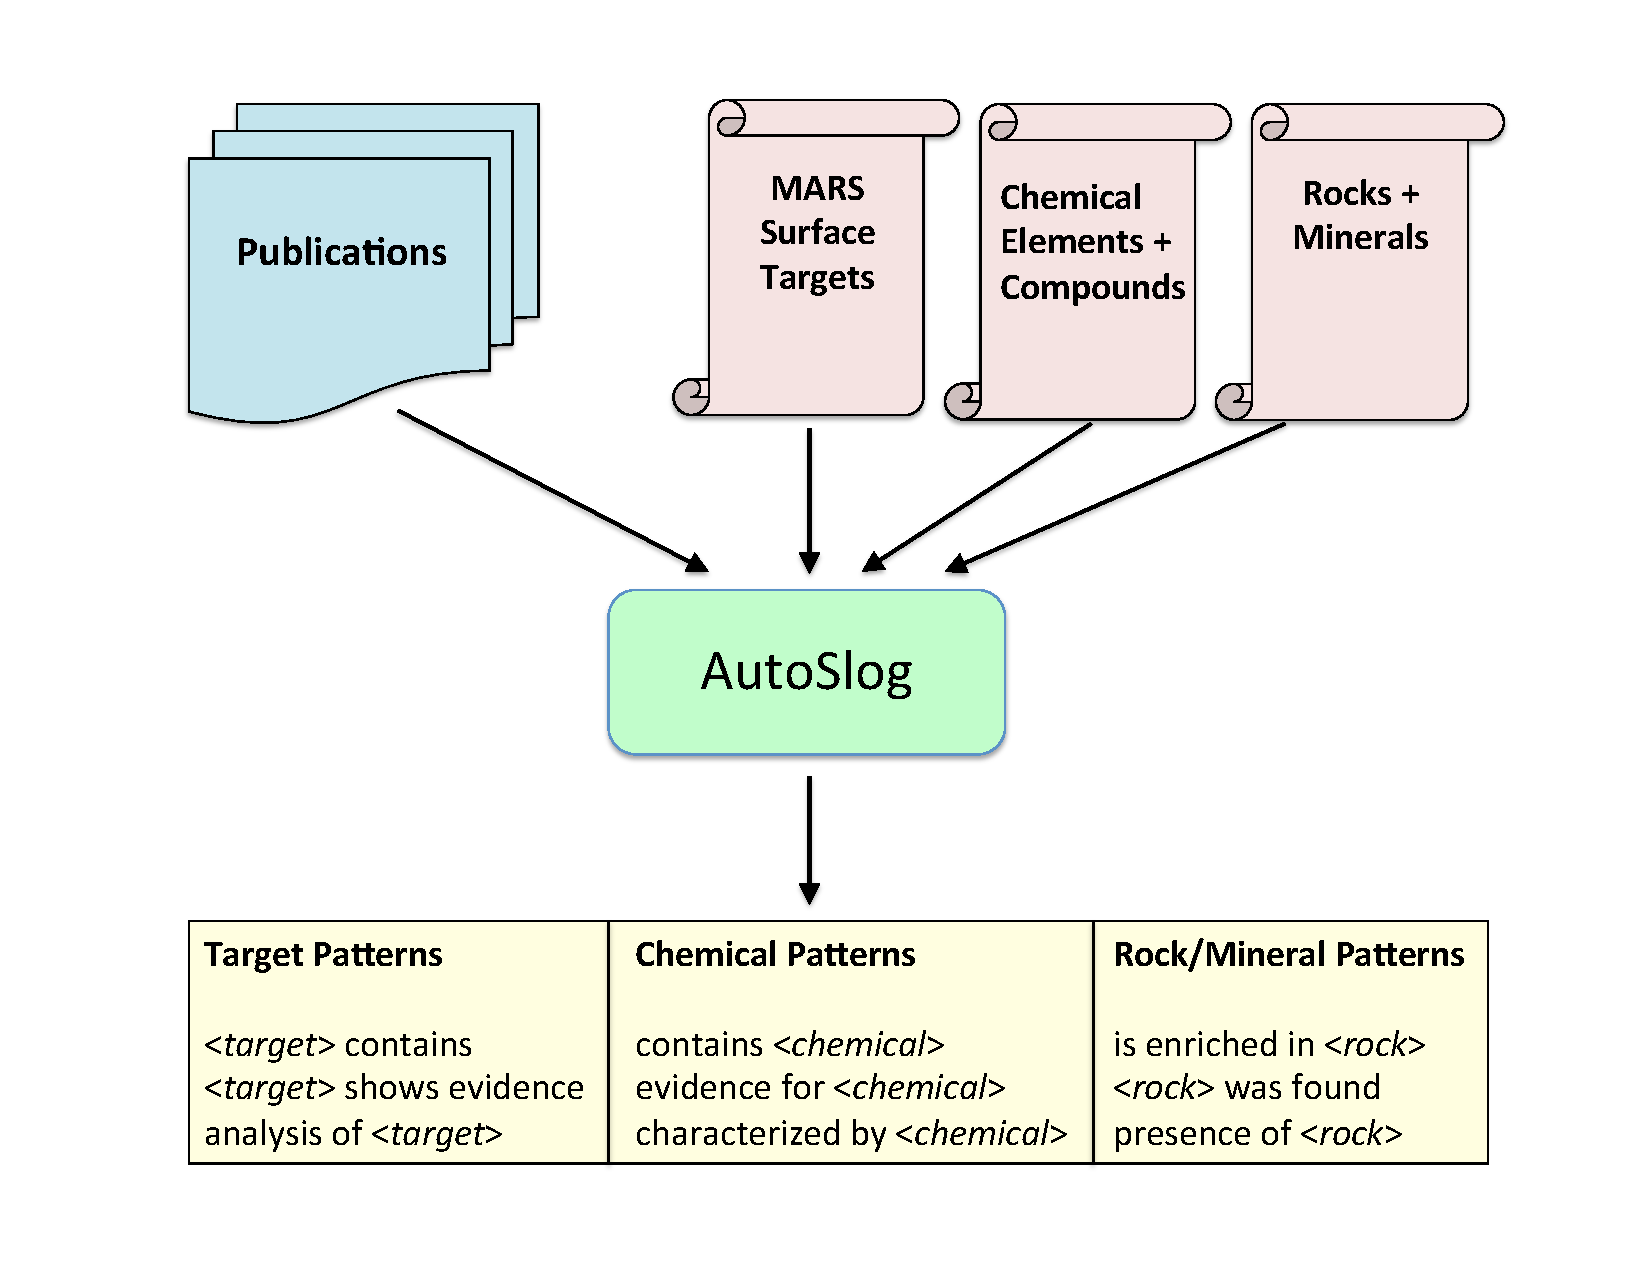
\includegraphics[width=3.5in]{fig/autoslog-pic.pdf}}
\caption{The extraction pattern generation process. AutoSlog learns
patterns from publications and lists of target names, chemical
elements and compounds, rocks, and minerals.}
\label{fig:ie}
\end{figure}

% EMR
The planetary science literature is large, providing us with an
abundance of text for this domain.  However, annotated texts are not
readily available, and obtaining human annotations from planetary
science experts would be time-consuming and expensive.  Our goal is
to design an information extraction (IE) process that uses weakly
supervised learning methods to extract knowledge from planetary
science articles.  

Figure~\ref{fig:ie} depicts the first step in our information
extraction process.  As input, we provide a text corpus of
publications along with lists of terms for relevant semantic
categories, such as ChemCam Mars surface target names, chemical
elements/compounds, and rocks/minerals. The AutoSlog extraction
pattern 
generator~\cite{riloff:autoslog93,riloff:autoslog96} is applied to
each list, producing a set of lexico-syntactic patterns associated
with the corresponding semantic category.  AutoSlog is a weakly
supervised pattern learner that uses heuristic rules and coarse
statistics, without requiring annotated documents. The learned
patterns can then be applied to new texts, to extract information that
we will store in the MTE. 

The AutoSlog software package includes the Sundance shallow
parser and information extraction engine~\cite{riloff:sundance04},
which applies the lexico-syntactic patterns generated by AutoSlog. 
The Sundance parser performs tokenization, sentence
segmentation, morphological analysis, part-of-speech disambiguation,
syntactic chunking, syntactic role assignment, and clause
segmentation. 
Although it was originally designed to process news articles, Sundance
has also been successfully applied to scientific publications from 
the biomedical literature~\cite{ramakrishnan:bio10,pokkunuri:bio11}.
A key attribute of Sundance is that its dictionaries and data
files are easily customizable for specialized domains, which has
allowed us to tailor it for planetary science texts. 
Our domain-specific customizations include (1) the specification of
two words that, despite ending in a period, do not indicate the end of
a sentence (``Mt.'' and ``wt.'') and (2) domain-specific vocabulary
including element names (e.g., ``chlorine'', ``Cl''), mineral names
(e.g., ``akaganeite'', ``feldspar'', ``MnO''), target names (from the
list described above), and unusual terms (e.g., ``sol'' (Martian day),
``MSL''). 

\subsection{Illustrative Results}

In this section, we provide example results for extracting
information for a Mars surface target named Windjana.  Windjana is a
sandstone that was named after the Windjana Gorge in Western
Australia~\cite{anderson:pads15}. 
% Cite paper 2417; this paper also has an nice image we could use

% todo: show parse output?
%{\bf [Here we could show parse output (if that level of detail is
%desired) and walk through one or more of 
%these examples.  Which one(s) should we use?]}

Consider the following four sentences, taken from different documents,
and the extraction patterns generated by AutoSlog using the target,
chemical, and mineral lists:

1: {\em ``Windjana is remarkable in containing an abundance of potassium
feldspar (and thus K in its bulk chemistry) combined with a low
abundance of plagioclase (and low Na/K in its chemistry).''} \\
% cite paper 2620
%AutoSlog extracts:
\centerline{
\begin{tabular}{|ll|} \hline 
Target:  & {\tt <subj>\_CONTAINING\_ABUNDANCE} \\
%(of potassium feldspar, of plagioclase)
Mineral: & {\tt ABUNDANCE\_OF\_<np>} \\
\hline
\end{tabular} 
}

%{\em ``As in other rock samples analyzed by CheMin, Windjana contains
%significant proportions of phyllosilicates and amorphous material.''}
% cite paper 2620
%AutoSlog extracts:
%Target: {\tt <subj>\_CONTAINS\_PROPORTIONS} \\
%(of phyllosilicates and amorphous material)
% had to add 'material' to get it to create this one
%{\tt PROPORTIONS\_OF\_<np>}

2: {\em ``The high abundances of K-feldspar and iron oxides in Windjana, also
reflected in the APXS chemical analysis as high K and Fe (Table 2)
[7], are unusual.''} \\
% cite paper 2620 treiman:windjana15
%AutoSlog extracts:
\centerline{
\begin{tabular}{|ll|} \hline 
Mineral: & {\tt ABUNDANCE\_OF\_<np>} \\ 
Target:  & {\tt OXIDES\_IN\_<subj>} \\
%(K-feldspar and iron) 
\hline
\end{tabular} 
}

3: {\em ``The Windjana sandstone contains high magnetite along with 2:1
phyllosilicates [9].''} \\
% cite paper 2971
%AutoSlog extracts:
\centerline{
\begin{tabular}{|ll|} \hline 
Target/Mineral: & {\tt <subj>\_CONTAINS\_MAGNETITE}  \\
\hline
\end{tabular} 
}
% need to know high/low!
%{\bf [Note: this example is interesting because the fact that it
%contains ``high'' magnetite is important (vs. ``low'' magnetite),
%i.e., the adjective matters.  What should we do about that?  Is this a
%future work topic?  Cardinality?  Could go with the epistemic bit
%mentioned later?]}

4: {\em ``The abundance of K-spar and the potential presence of illite in
Windjana must be considered when interpreting the formation of the
Dillinger sandstone because these phases can form in diagenetic K-rich
environments on Earth.''} \\
% cite paper 2038 rampe:cement15
%AutoSlog extracts:
\centerline{
\begin{tabular}{|ll|} \hline 
Mineral: & {\tt ABUNDANCE\_OF\_<np>} \\ 
Target/Mineral:  & {\tt ILLITE\_IN\_<np>} \\
\hline
\end{tabular} 
}

If we synthesize all the information found in these sentences by the
patterns, we can produce a summary of known properties about
Windjana:
%{\bf [show summary and discuss it - synthesizes knowledge from X
%different papers/authors into a single summary]}

\centerline{
\begin{tabular}{|p{2.75in}|} \hline
\multicolumn{1}{|c|}{Target Windjana} \\ \hline
Properties: \\
- contains abundance of potassium feldspar \\
- high abundances of K-feldspar and iron oxides \\
%- contains low abundance of plagioclase \\ % this wasn't successfully extracted
%- contains significant proportions of phyllosilicates and amorphous material \\
- contains high magnetite \\
- contains illite \\
\hline
\end{tabular}
}

% EMR: maybe need another sentence or two acknowledging that more steps
% will be needed to merge the info from different patterns?
The synthesis was done manually in this example, and we plan to
develop methods for merging the information extracted from different
patterns automatically.

This summary compiles knowledge extracted from multiple papers.
% Well, three papers.
While each author team might choose to focus on different aspects in
their individual papers, information extraction from the corpus as a
whole enables a collective picture of the composition of this target
to emerge.  This summary could inspire further discoveries or
hypotheses, as the reader considers, for example, what it means for
feldspar, magnetite, and illite to be jointly present and whether this
is unusual.

\section{Challenges}

In addition to the typical challenges of conducting information
extraction in a new domain (e.g.,~domain-specific vocabulary), there
are several NLP/IE challenges of special interest involved in this
project. 

%First, there is a need to combine case frames due to complex sentence
%structure.  {\bf [hopefully we can address this, at least in example
%form, above.  Or, we could keep the above examples simple and discuss
%it here.]}
%{\bf [Can we imagine how to handle cases like this:]} 
%{\em``strong enrichment in Zn on Windjana drill fines''}

First, we 
%must devise an appropriate and informative method for
%continually evaluating system performance.  
must maintain high precision in the extracted information.
For this application, precision is more important than recall; users
would rather have an incomplete summary than one that contains
incorrect information. 
Previous work on high-precision IE has emphasized the importance of
human review~\cite{caruana:hpie00}.  The AutoSlog-TS system 
ranks candidate extraction patterns based on their
prevalence in a set of (unannotated) relevant versus irrelevant
documents, enabling human review to be focused on the most likely
patterns first~\cite{riloff:autoslog96}.
This process also provides an assessment of the system's current
precision in extracting patterns.
We plan to likewise incorporate weak supervision via human review of
the extracted patterns and properties.

Second, we must identify and handle cases where the extracted
information within a summary is not consistent.  If the system
extracts a pair of properties such as ``high in magnetite'' and ``low
in magnetite'', for the same target, the consistency of the collective
result is reduced.
%
In some cases, it is non-trivial to determine whether two facts are
consistent or contradictory.  For example, consider two hypothetical
sentences: ``Target Oliphaunt is feldspar-rich'' and ``Target Oliphaunt has
low Si.''  By definition, a feldspar contains a lot of silicon, but
domain knowledge is required to detect that these statements are in
conflict.  

When contradictions are detected, we must determine how to reconcile
them.  The MTE inherently requires robust {\em information fusion} to
generate each encyclopedia entry.  Conflicts are especially likely
since the information is extracted from different authors and
publications rather than a single source.  Existing approaches to
cross-document information fusion include assigning a confidence
proportional to the number of sources that agree on a fact and
estimating the reliability of the sources
themselves~\cite{ji:infofusion10}.

% EMR: this isn't really an NLP issue per se, and not unique to this
% domain,  so could be omitted.  
%% Third, the MTE database of extracted information must be updated
%% frequently, because (1) the list of Mars surface target names is
%% continually growing and (2) the volume of relevant publications also
%% grows.  In all scientific endeavors, knowledge evolves and some of it
%% becomes outdated.  An interpretation could be overturned or negated by
%% later findings or a more careful examination of the available data.
Since there is a temporal component to the papers, it can also be the
case that an interpretation could be overturned or negated by later
findings or a more careful examination of the available data.  The
same challenge appears when performing information extraction for 
news articles~\cite{mckeown:news95,ji:infofusion10}
%{\bf [include cites here / discuss how others address
%this issue]}.
%
A simple strategy would be to let the most recently reported
information, as determined by publication date, supersede older
information.  However, since apparent conflicts could be created by an
incorrect extraction (see above), it may be best to flag the facts as
conflicting but let the user review them. 

Third, coreference is especially challenging because of the diversity
in how authors refer to the same targets or properties.  Windjana is
variously referred to as ``Windjana'', ``Windjana drill fines'',
``Windjana drill tailings'', ``Windjana sample'', ``Windjana
sandstone'', ``it'', etc.  Elements and minerals have multiple
manifestations; ``Cl'' vs. ``chlorine'', ``potassium feldspar''
vs. ``K-feldspar'' vs. ``K-spar'', etc.  Coreference resolution
remains an unsolved problem, although new advances in active learning
are promising~\cite{sachan:coref15}.

% EMR: NLP folks will find this interesting. I think it's related to
% work on "hedging" ... I'll try to find some citations.
Fourth, when interpreting observations, scientific conclusions range
from solid facts to speculation about causes.  In some cases, evidence
even for basic properties (e.g., ``contains Mn'') may fall into a gray
area.  Scientific language may therefore employ epistemic modifiers
such as ``likely'' or ``probably'' or ``possibly.''  Examples from the
LPSC 2015 corpus related to the Windjana target include {\em ``the
Windjana drill tailings likely contain a spectrally opaque material
(e.g., magnetite, ilmenite)''}~\cite{johnson:ferric15} and {\em ``the
potential presence of illite in Windjana''}~\cite{rampe:cement15}.
This type of language is known as {\em hedging}, and some methods have
been developed for automatically detecting
hedges~\cite{medlock:hedge07,agarwal:hedge10}.  
% Note: HedgeScope
% (http://hedgescope.askhermes.org/hedgescope/index.php)
% detects hedging in the first example but not the second
% (had to specify 'Clinical' type to get a detection)
Distinguishing this information from more confidently stated
conclusions is vital to preserving the nuance reported in the
documents, as previously studied in the context of medical discussion
forums~\cite{sokolova:epistemic13}.
%
%{\bf [Could also build on Ellen's previous work on subjective
%  expressions?  (EMNLP 2003)]}

\section{Conclusions and Next Steps}

There is a growing need for a comprehensive, up-to-date compilation of
Mars surface targets and knowledge of what has been discovered about
them.  We are working to automatically construct a Mars Target
Encyclopedia by applying information extraction methods to planetary
science publications.  This is a cross-document information extraction
task that will benefit ongoing science investigations by providing the
full context of previously published knowledge.  Browsing the
synthesized encyclopedia entries, with their summaries of target
knowledge, could also reveal previously undetected connections or
similarities between targets. 

% We have not yet addressed the issue of coreference.

We have employed Tika, Sundance, and AutoSlog to extract basic
information about Mars surface targets.  We plan to employ a small
amount of human review to provide light supervision/feedback and
evaluation of the system's precision.
%
Important open questions remain about how to detect and accommodate
inconsistency in information extracted from different documents at
different times.  The system also must correctly capture epistemic
modifiers so that the level of confidence in the extracted knowledge
is preserved.

%What is the role of supervision? Some human review of extracted info -
%are any annotations needed? 

%Describe larger planned system (store extracted information in a
%Solr database, use JSON to generate MTE webpages)?

The initial term lists that we give to AutoSlog were manually
compiled, but we plan to expand them automatically using bootstrapping
methods for semantic lexicon induction. The goal is to learn
additional terms that can refer to Mars targets, chemicals, and
rocks/minerals, such as missing terms (because manually compiled lists
are inevitably incomplete) as well as name variants (e.g.,
``World-beater'' vs. ``Worldbeater''), general terms (e.g.,
``target''), abbreviations (e.g., ``F'' for fluorine), and shorthand
terms (e.g., ``Fe-oxide'' vs. ``iron oxide'').  We will use the
Basilisk semantic lexicon bootstrapping
algorithm~\cite{thelen:basilisk02}, using the manually compiled lists
as seed terms and a large collection of planetary science articles as
the text corpus. Basilisk automatically learns new semantic class
members by identifying terms that consistently co-occur in related
contexts with the seeds, in an iterative bootstrapping process.
Basilisk has been successfully used to generate semantic dictionaries
for a variety of domains, including disease
outbreaks~\cite{phillips:role07,qadir:ens12}, terrorist
events~\cite{thelen:basilisk02}, and subjectivity
analysis~\cite{riloff:subj03}. We will manually review Basilisk's
proposed additions to maintain high integrity of the lists.

%We will expand to include more text sources and ultimately targets
%from other instruments/missions.

In addition to these plans, we welcome suggestions that can help guide
the evolution and maturation of the MTE to maximize its utility and
impact.

\section*{Acknowledgments}
This work was carried out in part at the Jet Propulsion Laboratory,
California Institute of Technology, under a contract with the National
Aeronautics and Space Administration. Government sponsorship
acknowledged.

\bibliography{mte}
\bibliographystyle{aaai}

\end{document}

% LocalWords:  aaai sty AAAI Kiri Wagstaff CA Lanza Los Riloff UT Mattmann Tika
% LocalWords:  Sundance AutoSlog EMR genomic MTE Epworth Frood Worldbeater MSL
% LocalWords:  XXXX YYYY ChemCam NLP IE LPSC Todo PDF lexico tokenization Mt wt
% LocalWords:  chunking Cl akaganeite MnO sol Windjana todo Na subj np CheMin
% LocalWords:  phyllosilicates APXS Fe treiman windjana epistemic illite rampe
% LocalWords:  diagenetic Zn TS Si se coreference Mn ilmenite HedgeScope EMNLP
% LocalWords:  Solr JSON webpages co mte
